Afin de calculer le pourcentage de lignes dupliquées, nous avons créé
une nouvelle table, contenant les noms des programmes, leurs
domaines, les langages dans lesquels ils ont été écrits et leurs
nombres de lignes dupliquées (figure \ref{fig:dlin_prog}) ainsi que
leurs nombres de lignes totales. Nous avons enlevé de cette nouvelle
table de données les programmes ayant un champ non renseigné (à
l'aide de la commande \lstinline{na.omit}). Nous avons ensuite rajouté une
colonne à celle-ci contenant les pourcentages de lignes de code
dupliquées, avant de créer un histogramme de ces pourcentages pour
chaque programme, ordonné par ordre décroissant (figure
\ref{fig:pdlin_prog}).

\begin{figure}[h]
  \minipage{0.48\textwidth}
  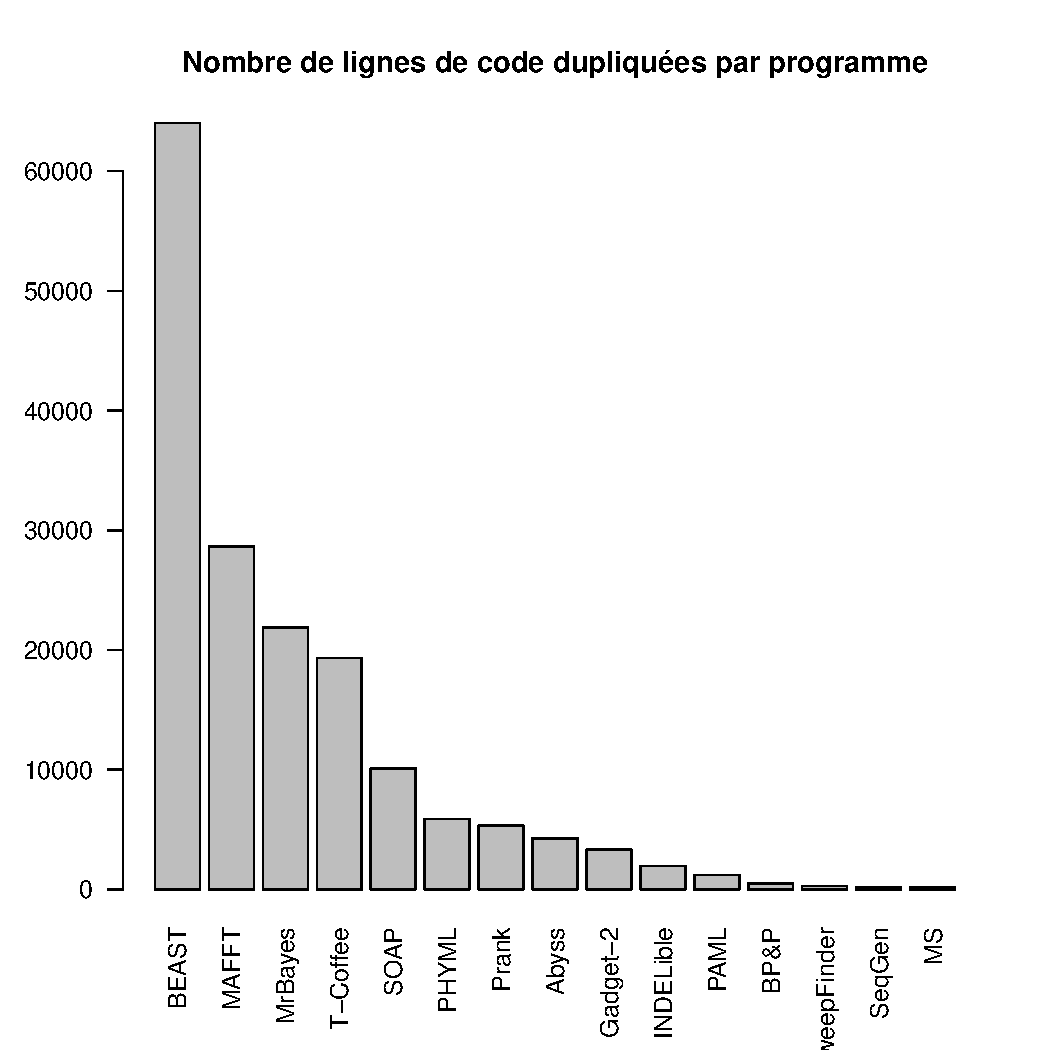
\includegraphics[width=\linewidth]{figures/dlin_prog.pdf}
  \caption{}\label{fig:dlin_prog}
  \endminipage\hfill
  \minipage{0.48\textwidth}
  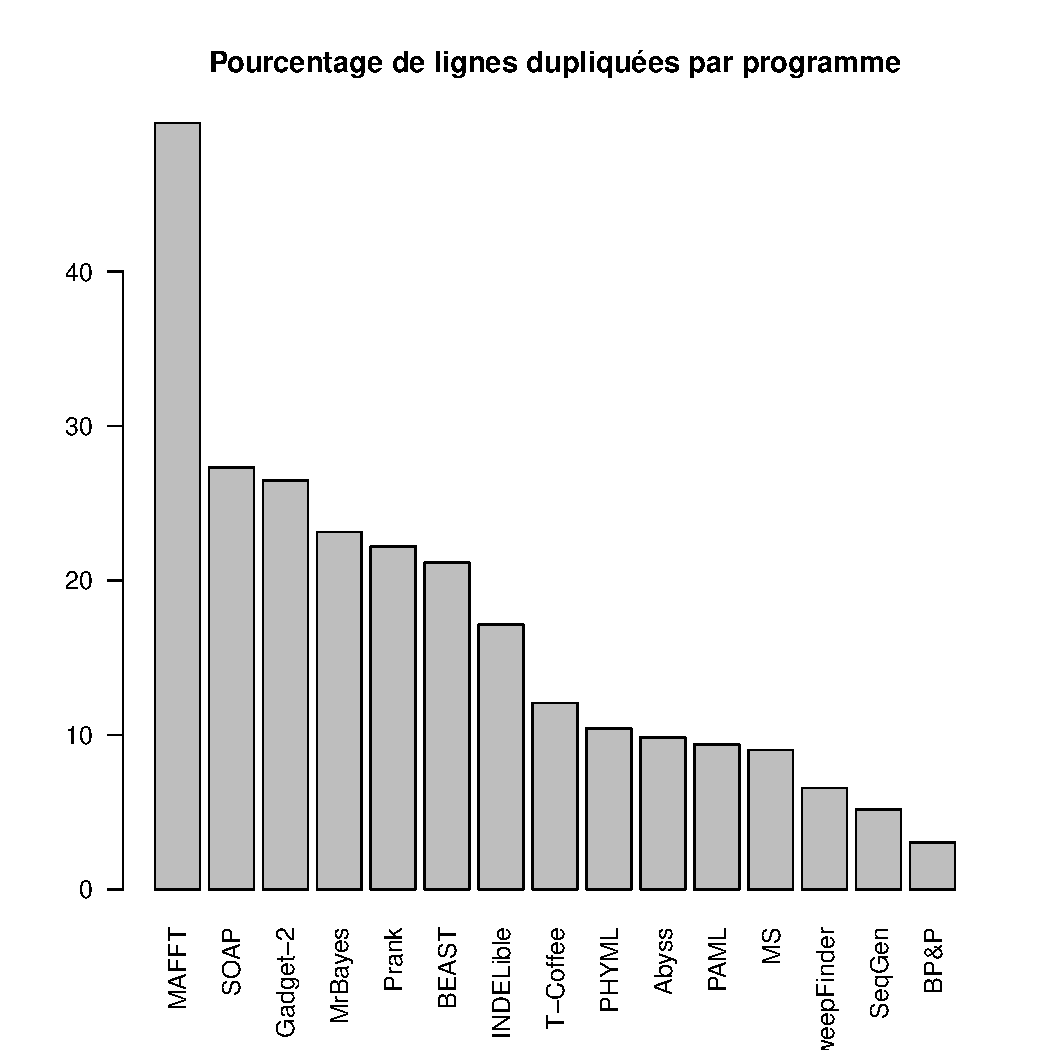
\includegraphics[width=\linewidth]{figures/pdlin_prog.pdf}
  \caption{}\label{fig:pdlin_prog}
  \endminipage\hfill
\end{figure}
